%%
% Copyright (c) 2017 - 2019, Pascal Wagler;  
% Copyright (c) 2014 - 2019, John MacFarlane
% 
% All rights reserved.
% 
% Redistribution and use in source and binary forms, with or without 
% modification, are permitted provided that the following conditions 
% are met:
% 
% - Redistributions of source code must retain the above copyright 
% notice, this list of conditions and the following disclaimer.
% 
% - Redistributions in binary form must reproduce the above copyright 
% notice, this list of conditions and the following disclaimer in the 
% documentation and/or other materials provided with the distribution.
% 
% - Neither the name of John MacFarlane nor the names of other 
% contributors may be used to endorse or promote products derived 
% from this software without specific prior written permission.
% 
% THIS SOFTWARE IS PROVIDED BY THE COPYRIGHT HOLDERS AND CONTRIBUTORS 
% "AS IS" AND ANY EXPRESS OR IMPLIED WARRANTIES, INCLUDING, BUT NOT 
% LIMITED TO, THE IMPLIED WARRANTIES OF MERCHANTABILITY AND FITNESS 
% FOR A PARTICULAR PURPOSE ARE DISCLAIMED. IN NO EVENT SHALL THE 
% COPYRIGHT OWNER OR CONTRIBUTORS BE LIABLE FOR ANY DIRECT, INDIRECT, 
% INCIDENTAL, SPECIAL, EXEMPLARY, OR CONSEQUENTIAL DAMAGES (INCLUDING,
% BUT NOT LIMITED TO, PROCUREMENT OF SUBSTITUTE GOODS OR SERVICES; 
% LOSS OF USE, DATA, OR PROFITS; OR BUSINESS INTERRUPTION) HOWEVER 
% CAUSED AND ON ANY THEORY OF LIABILITY, WHETHER IN CONTRACT, STRICT 
% LIABILITY, OR TORT (INCLUDING NEGLIGENCE OR OTHERWISE) ARISING IN 
% ANY WAY OUT OF THE USE OF THIS SOFTWARE, EVEN IF ADVISED OF THE 
% POSSIBILITY OF SUCH DAMAGE.
%%

%%
% This is the Eisvogel pandoc LaTeX template.
%
% For usage information and examples visit the official GitHub page:
% https://github.com/Wandmalfarbe/pandoc-latex-template
%%

% Options for packages loaded elsewhere
\PassOptionsToPackage{unicode}{hyperref}
\PassOptionsToPackage{hyphens}{url}
\PassOptionsToPackage{dvipsnames,svgnames*,x11names*,table}{xcolor}
%
\documentclass[
  english,
  a4paper,
,tablecaptionabove
]{scrartcl}
\usepackage{lmodern}
\usepackage{setspace}
\setstretch{1.2}
\usepackage{amssymb,amsmath}
\usepackage{ifxetex,ifluatex}
\ifnum 0\ifxetex 1\fi\ifluatex 1\fi=0 % if pdftex
  \usepackage[T1]{fontenc}
  \usepackage[utf8]{inputenc}
  \usepackage{textcomp} % provide euro and other symbols
\else % if luatex or xetex
  \usepackage{unicode-math}
  \defaultfontfeatures{Scale=MatchLowercase}
  \defaultfontfeatures[\rmfamily]{Ligatures=TeX,Scale=1}
\fi
% Use upquote if available, for straight quotes in verbatim environments
\IfFileExists{upquote.sty}{\usepackage{upquote}}{}
\IfFileExists{microtype.sty}{% use microtype if available
  \usepackage[]{microtype}
  \UseMicrotypeSet[protrusion]{basicmath} % disable protrusion for tt fonts
}{}
\makeatletter
\@ifundefined{KOMAClassName}{% if non-KOMA class
  \IfFileExists{parskip.sty}{%
    \usepackage{parskip}
  }{% else
    \setlength{\parindent}{0pt}
    \setlength{\parskip}{6pt plus 2pt minus 1pt}}
}{% if KOMA class
  \KOMAoptions{parskip=half}}
\makeatother
\usepackage{xcolor}
\definecolor{default-linkcolor}{HTML}{A50000}
\definecolor{default-filecolor}{HTML}{A50000}
\definecolor{default-citecolor}{HTML}{4077C0}
\definecolor{default-urlcolor}{HTML}{4077C0}
\IfFileExists{xurl.sty}{\usepackage{xurl}}{} % add URL line breaks if available
\IfFileExists{bookmark.sty}{\usepackage{bookmark}}{\usepackage{hyperref}}
\hypersetup{
  pdftitle={PPM Project Report - Group Kii},
  pdfauthor={Callum Axon (N0727303); Callum Carney (N0741707); Jordan Brightmore (N0732961); Finlay McKinnon (N0743587); Vital Harachka (N0731739); Wing Chiang (T0086366)},
  colorlinks=true,
  linkcolor=darkgray,
  filecolor=default-filecolor,
  citecolor=default-citecolor,
  urlcolor=default-urlcolor,
  breaklinks=true,
  pdfcreator={LaTeX via pandoc with the Eisvogel template}}
\urlstyle{same} % disable monospaced font for URLs
\usepackage[margin=2.5cm,includehead=true,includefoot=true,centering]{geometry}
\usepackage[export]{adjustbox}
\usepackage{graphicx}
\usepackage{longtable,booktabs}
% Correct order of tables after \paragraph or \subparagraph
\usepackage{etoolbox}
\makeatletter
\patchcmd\longtable{\par}{\if@noskipsec\mbox{}\fi\par}{}{}
\makeatother
% Allow footnotes in longtable head/foot
\IfFileExists{footnotehyper.sty}{\usepackage{footnotehyper}}{\usepackage{footnote}}
\makesavenoteenv{longtable}
\usepackage{graphicx,grffile}
\makeatletter
\def\maxwidth{\ifdim\Gin@nat@width>\linewidth\linewidth\else\Gin@nat@width\fi}
\def\maxheight{\ifdim\Gin@nat@height>\textheight\textheight\else\Gin@nat@height\fi}
\makeatother
% Scale images if necessary, so that they will not overflow the page
% margins by default, and it is still possible to overwrite the defaults
% using explicit options in \includegraphics[width, height, ...]{}
\setkeys{Gin}{width=\maxwidth,height=\maxheight,keepaspectratio}
\setlength{\emergencystretch}{3em}  % prevent overfull lines
\providecommand{\tightlist}{%
  \setlength{\itemsep}{0pt}\setlength{\parskip}{0pt}}
\setcounter{secnumdepth}{-\maxdimen} % remove section numbering

% Make use of float-package and set default placement for figures to H
\usepackage{float}
\floatplacement{figure}{H}

\usepackage{pdflscape}
\ifxetex
    % See issue https://github.com/reutenauer/polyglossia/issues/127
  \renewcommand*\familydefault{\sfdefault}
  % Load polyglossia as late as possible: uses bidi with RTL langages (e.g. Hebrew, Arabic)
  \usepackage{polyglossia}
  \setmainlanguage[]{english}
\else
  \usepackage[shorthands=off,main=english]{babel}
\fi

\title{PPM Project Report - Group Kii}
\usepackage{etoolbox}
\makeatletter
\providecommand{\subtitle}[1]{% add subtitle to \maketitle
  \apptocmd{\@title}{\par {\large #1 \par}}{}{}
}
\makeatother
\subtitle{Magnus Frater System}
\author{Callum Axon (N0727303) \and Callum Carney (N0741707) \and Jordan Brightmore (N0732961) \and Finlay McKinnon (N0743587) \and Vital Harachka (N0731739) \and Wing Chiang (T0086366)}
\date{}





%%
%% added
%%

%
% language specification
%
% If no language is specified, use English as the default main document language.
%


%
% for the background color of the title page
%
\usepackage{pagecolor}
\usepackage{afterpage}

%
% break urls
%
\PassOptionsToPackage{hyphens}{url}

%
% When using babel or polyglossia with biblatex, loading csquotes is recommended 
% to ensure that quoted texts are typeset according to the rules of your main language.
%
\usepackage{csquotes}

%
% captions
%
\definecolor{caption-color}{HTML}{777777}
\usepackage[font={stretch=1.2}, textfont={color=caption-color}, position=top, skip=4mm, labelfont=bf, singlelinecheck=false, justification=raggedright]{caption}
\setcapindent{0em}

%
% blockquote
%
\definecolor{blockquote-border}{RGB}{221,221,221}
\definecolor{blockquote-text}{RGB}{119,119,119}
\usepackage{mdframed}
\newmdenv[rightline=false,bottomline=false,topline=false,linewidth=3pt,linecolor=blockquote-border,skipabove=\parskip]{customblockquote}
\renewenvironment{quote}{\begin{customblockquote}\list{}{\rightmargin=0em\leftmargin=0em}%
\item\relax\color{blockquote-text}\ignorespaces}{\unskip\unskip\endlist\end{customblockquote}}

%
% Source Sans Pro as the de­fault font fam­ily
% Source Code Pro for monospace text
%
% 'default' option sets the default 
% font family to Source Sans Pro, not \sfdefault.
%
\usepackage[default]{sourcesanspro}
\usepackage{sourcecodepro}

% XeLaTeX specific adjustments for straight quotes: https://tex.stackexchange.com/a/354887
% This issue is already fixed (see https://github.com/silkeh/latex-sourcecodepro/pull/5) but the 
% fix is still unreleased.
% TODO: Remove this workaround when the new version of sourcecodepro is released on CTAN.
\ifxetex
\makeatletter
\defaultfontfeatures[\ttfamily]
  { Numbers   = \sourcecodepro@figurestyle,
    Scale     = \SourceCodePro@scale,
    Extension = .otf }
\setmonofont
  [ UprightFont    = *-\sourcecodepro@regstyle,
    ItalicFont     = *-\sourcecodepro@regstyle It,
    BoldFont       = *-\sourcecodepro@boldstyle,
    BoldItalicFont = *-\sourcecodepro@boldstyle It ]
  {SourceCodePro}
\makeatother
\fi

%
% heading color
%
\definecolor{heading-color}{RGB}{40,40,40}
\addtokomafont{section}{\color{heading-color}}
% When using the classes report, scrreprt, book, 
% scrbook or memoir, uncomment the following line.
%\addtokomafont{chapter}{\color{heading-color}}

%
% variables for title and author
%
\usepackage{titling}
\title{PPM Project Report - Group Kii}
\author{Callum Axon (N0727303), Callum Carney (N0741707), Jordan Brightmore (N0732961), Finlay McKinnon (N0743587), Vital Harachka (N0731739), Wing Chiang (T0086366)}

%
% tables
%

\definecolor{table-row-color}{HTML}{F5F5F5}
\definecolor{table-rule-color}{HTML}{999999}

%\arrayrulecolor{black!40}
\arrayrulecolor{table-rule-color}     % color of \toprule, \midrule, \bottomrule
\setlength\heavyrulewidth{0.3ex}      % thickness of \toprule, \bottomrule
\renewcommand{\arraystretch}{1.3}     % spacing (padding)

% Reset rownum counter so that each table
% starts with the same row colors.
% https://tex.stackexchange.com/questions/170637/restarting-rowcolors
\let\oldlongtable\longtable
\let\endoldlongtable\endlongtable
\renewenvironment{longtable}{
\rowcolors{3}{}{table-row-color!100}  % row color
\oldlongtable} {
\endoldlongtable
\global\rownum=0\relax}

% Unfortunately the colored cells extend beyond the edge of the 
% table because pandoc uses @-expressions (@{}) like so: 
%
% \begin{longtable}[]{@{}ll@{}}
% \end{longtable}
%
% https://en.wikibooks.org/wiki/LaTeX/Tables#.40-expressions

%
% remove paragraph indention
%
\setlength{\parindent}{0pt}
\setlength{\parskip}{6pt plus 2pt minus 1pt}
\setlength{\emergencystretch}{3em}  % prevent overfull lines

%
%
% Listings
%
%


%
% header and footer
%
\usepackage{fancyhdr}

\fancypagestyle{eisvogel-header-footer}{
  \fancyhead{}
  \fancyfoot{}
  \lhead[]{PPM Project Report - Group Kii}
  \chead[]{}
  \rhead[PPM Project Report - Group Kii]{}
  \lfoot[\thepage]{Callum Axon (N0727303), Callum Carney (N0741707), Jordan Brightmore (N0732961), Finlay McKinnon (N0743587), Vital Harachka (N0731739), Wing Chiang (T0086366)}
  \cfoot[]{}
  \rfoot[Callum Axon (N0727303), Callum Carney (N0741707), Jordan Brightmore (N0732961), Finlay McKinnon (N0743587), Vital Harachka (N0731739), Wing Chiang (T0086366)]{\thepage}
  \renewcommand{\headrulewidth}{0.4pt}
  \renewcommand{\footrulewidth}{0.4pt}
}
\pagestyle{eisvogel-header-footer}

%%
%% end added
%%

\begin{document}

%%
%% begin titlepage
%%

\begin{titlepage}
\newgeometry{left=6cm}
\definecolor{titlepage-color}{HTML}{06386e}
\newpagecolor{titlepage-color}\afterpage{\restorepagecolor}
\newcommand{\colorRule}[3][black]{\textcolor[HTML]{#1}{\rule{#2}{#3}}}
\begin{flushleft}
\noindent
\\[-1em]
\color[HTML]{FFFFFF}
\makebox[0pt][l]{\colorRule[FFFFFF]{1.3\textwidth}{1pt}}
\par
\noindent

{ \setstretch{1.4}
\vfill
\noindent {\huge \textbf{\textsf{PPM Project Report - Group Kii}}}
\vskip 1em
{\Large \textsf{Magnus Frater System}}
\vskip 2em
\noindent
{\Large \textsf{Callum Axon (N0727303), Callum Carney (N0741707), Jordan Brightmore (N0732961), Finlay McKinnon (N0743587), Vital Harachka (N0731739), Wing Chiang (T0086366)}
\vfill
}

\noindent

\includegraphics[width=60pt, left]{./images/ntu-logo.png}

\textsf{}}
\end{flushleft}
\end{titlepage}
\restoregeometry

%%
%% end titlepage
%%



\hypertarget{abstract}{%
\section{Abstract}\label{abstract}}

Magnus Frater (or Big Brother) has been created to help tackle the
ongoing issue of security within large open campuses and premises, these
sorts of locations inherently have an increased potential for intrusion
through unmonitored sections of land. The group analysed the recent
spree of attacks on schools and offices - for example the shooting that
occurred at the YouTube headquarters in 2018 (Staff and Agencies 2018) -
and found that in a large amount of these attacks there were open doors
and spaces that allowed the attacker to enter with ease. As a
consequence to this, the idea of creating a facial recognition system to
analyse and report known and unknown people within a campus/large open
setting was conceived.

As mentioned, the main purpose of the project was to create a system
that would accurately detect and report people walking around an area to
the associated security team, this data would differentiate between
employees or authorised users and unknown people by linking into the
companies employee/student database. Not only would this allow a
security team to monitor who is within a set area at any one time, but
it would also allow administrative users to track any persons movements
and activities within a set time frame, through tracking of the targets
face across multiple cameras. Another advantage to this project is that
administrative users can view analytics in relation to the usage of
campus properties, an example use case for this would be within a
University. Admins could check what buildings within the campus are
being utilised most by students.

After the main purpose behind the project was defined, the group decided
on how to proceed in regards to the requirements for the project, most
importantly how we should proceed with splitting up the individual
hardware and software components so that the system could functions
within any scenario or environment. It was decided that there will be 4
different modules, these being:

\begin{enumerate}
\def\labelenumi{\arabic{enumi}.}
\tightlist
\item
  A Raspberry Pi that would be responsible for processing any facial
  data that is captured by the camera
\item
  A Camera module that would connect directly to the Raspberry Pi and
  provide images to the Raspberry Pi
\item
  A website created for administrators and security personnel to
  administer and manage hits/rejections.
\item
  An API (Application Programming Interface) used within the website and
  the Raspberry Pi for collation and provision of data.
\end{enumerate}

These modules will work together to create the Cameras that report
facial data and the web interface that is used to manage the data
received by the camera, the connection between these modules was
outlined in the design documentation (for example the Data Flow Diagram
and Entity Relationship Diagram).

Once the components and requirements were completed, the group began to
consider which programming languages and setups would be best suited for
the type of project this is (Facial Recognition with Web Related
components). It was clear that Python should be used for the facial
recognition section of the project due to its strong existing libraries.
NodeJS would be used for the Web Frontend, PHP would be used to power
the backend API that links all of the components together and the API
would be using a MySQL database to hold all of the data. The system
would work in the following way:

\begin{enumerate}
\def\labelenumi{\arabic{enumi}.}
\tightlist
\item
  The Camera feeds data to the Raspberry Pi
\item
  The Python application on the Raspberry Pi calculates if a face is
  present
\item
  Any potential face found is sent to the API where corresponding facial
  data is requested from the database
\item
  If no corresponding data is found, then the face is unknown, otherwise
  the image will be linked to the person the face associates with.
\item
  The Website will update using data from the API to show new
  detections, known or unknown.
\end{enumerate}

Once the product had been developed, testing took place to ensure that
the facial recognition software worked from a variety of different
distances and in unfavourable circumstances (heavy rain, fog, etc).
While some of the tests passed, others failed to detect faces when they
were present, however this only occurred in extreme circumstances. We
made small enhancements to the facial detection algorithm to improve its
effectiveness during these scenarios.

Due to the nature of this system, there are a lot of potential legal and
ethical issues, people may not consent to the recording of their faces,
people may not wish to have their faces processed and stored by this
system. Therefore it was important for us to implement a blacklist
system that would stop the system from performing facial data
processing, however, this is a complex system because we first need to
process a persons face to understand what to blacklist, which could
cause further legal or ethical issues.

\newpage

\hypertarget{table-of-contents}{%
\section{Table of Contents}\label{table-of-contents}}

\begin{itemize}
\tightlist
\item
  \protect\hyperlink{abstract}{Abstract}
\item
  \protect\hyperlink{table-of-contents}{Table of Contents}
\item
  \protect\hyperlink{introduction}{Introduction}

  \begin{itemize}
  \tightlist
  \item
    \protect\hyperlink{aims}{Aims}
  \item
    \protect\hyperlink{objectives}{Objectives}
  \end{itemize}
\item
  \protect\hyperlink{project-management}{Project Management}

  \begin{itemize}
  \tightlist
  \item
    \protect\hyperlink{meetings}{Meetings}

    \begin{itemize}
    \tightlist
    \item
      \protect\hyperlink{general-absence}{General Absence}
    \item
      \protect\hyperlink{authorised-absence}{Authorised Absence}
    \item
      \protect\hyperlink{absence-procedure}{Absence Procedure}
    \end{itemize}
  \item
    \protect\hyperlink{management}{Management}

    \begin{itemize}
    \tightlist
    \item
      \protect\hyperlink{project-manager}{Project Manager}
    \item
      \protect\hyperlink{task-allocation}{Task Allocation}
    \end{itemize}
  \item
    \protect\hyperlink{team-members-responsibility--skills}{Team
    Members, Responsibility \& Skills}
  \end{itemize}
\item
  \protect\hyperlink{risk-assessment}{Risk Assessment}
\item
  \protect\hyperlink{requirements}{Requirements}

  \begin{itemize}
  \tightlist
  \item
    \protect\hyperlink{functional-requirements}{Functional Requirements}
  \item
    \protect\hyperlink{non-functional-requirements}{Non-Functional
    Requirements}
  \end{itemize}
\item
  \protect\hyperlink{normalisation}{Normalisation}
\item
  \protect\hyperlink{context-diagram}{Context Diagram}

  \begin{itemize}
  \tightlist
  \item
    \protect\hyperlink{bcs-code-of-conduct}{BCS Code of Conduct}
  \end{itemize}
\item
  \protect\hyperlink{references}{References}
\end{itemize}

\newpage

\hypertarget{introduction}{%
\section{Introduction}\label{introduction}}

\hypertarget{aims}{%
\subsection{Aims}\label{aims}}

The main aim of the project is to provide organisations with open campus
settings a way to effectively track and monitor who is on campus and
where they are located at any time of day. This is to help reduce or
prevent intrusions and attacks that occur on these types of locations.

\hypertarget{objectives}{%
\subsection{Objectives}\label{objectives}}

To ensure clear and appropriate objectives have been created for the
project, the S.M.A.R.T. (specific, measurable, achievable/appropriate,
realistic, time-constrained) goals (Doran 1981) were used. SMART allows
us to create objectives that provide the project with lots of
functionality, that will be meaningful to the objects, and still stay
within the projects deadlines. For the project to be successful the
following objectives should be met:

Staff Members should be able to:

\begin{itemize}
\tightlist
\item
  Add new faces or people to the system through a simple yet effective
  web interface
\item
  Monitor the movements of people across buildings and campuses, whether
  they are registered as people or not
\item
  Manage alerts of unknown people entering the campus
\item
  Provide temporary passes to unknown people to authorize them for a set
  amount of time;
\end{itemize}

As a requirement to this, the camera and associated Raspberry Pi module
should be able to provide the following:

\begin{itemize}
\tightlist
\item
  A stream of video that can be analysed by the algorithm on the Pi in
  order to find faces;
\item
  A constant stream of face detections to the central server that
  manages all hits;
\end{itemize}

In general the following objective should be met:

\begin{itemize}
\tightlist
\item
  The camera and web interface should be able to talk to each other
  through an API (Application Programming Interface)
\end{itemize}

To meet the objectives set out for Staff Members, the group will be
creating a web interface using NodeJS, this interface will have the
functionality set out above and will interface with the API to get and
set data. It was mentioned that the interface should be simple yet
effective, we could easily bombard the user with a lot of metadata from
the cameras, however, the web interface will only show the required
information and actions to ensure that a staff member can quickly and
easily identify if there is an intruder currently on campus. All of the
outlines objectives are achievable and can be implemented in a timely
manner.

To meet the requirements set out for the Raspberry Pi and API, we will
have to ensure substantial testing of the facial detection algorithm
takes place, the group wants to avoid experiencing a scenario in which
multiple people are not identified. However, the algorithm cannot be
100\% effective, there will always be scenarios in which the algorithm
misses a person, or mis-identifies them, it would be unrealistic and a
waste of development time to be chasing after a 100\% success rate. We
will also have to ensure that the API is tested thoroughly, not only for
functionality, but for security purposes, if an attacker gained access
to another users facial data then this would be a breach of GDPR,
therefore we will be implementing multiple security procedures to ensure
that the API is secure, including the use of security based unit testing
and manual testing.

\newpage

\hypertarget{project-management}{%
\section{Project Management}\label{project-management}}

\hypertarget{meetings}{%
\subsection{Meetings}\label{meetings}}

Group meetings should occur at least once a week during term time.This
may be altered and increased dependent on any deadlines that the group
decide are enough of an impact to call extra meetings. The current
meetings have an estimated length of 30 minutes to an hour, being held
in a work-appropriate environment, such as a meeting room. IT can be
useful to utilise software which allows the use of voice communication
to enable remote working. It is possible that there will be instances in
which not all the group will be able to meet. This may be caused through
a great many scenario, each of which should be able to be resolved,
given consideration and following a standard procedure. Some of the
scenarios, and correct procedures to take in the event of said scenario,
can be seen below:

\hypertarget{general-absence}{%
\subsubsection{General Absence}\label{general-absence}}

In the case of a general absence, being that a member of the group is
absent without meaningful reason, the group may have to consider the
situation the absent member may be in. The consideration being the
current group position, the importance of the absent member's role, or
contribution that may have been needed in the current session. In this
event, the group may need to note down the general absence and keep
track of the amount each member has committed, as many of these may show
a lack of commitment to the project. A given example of this scenario is
- ''Marcus missed the meeting because he went to go see a movie.''

\hypertarget{authorised-absence}{%
\subsubsection{Authorised Absence}\label{authorised-absence}}

In the event of an authorised absence, in which the member who is absent
has given compelling reason and possibly proof if required, the member
would be excused from the current session. For this scenario to be
distinguishable from a general absence is down to a few possibilities:
forewarning of absence with given reasoning and a group consensus to
pass this absence, an event in which the member would not be able to
attend due to reasoning outside of their control, or an unavoidable
event where the member has no real ability to alter A given example of
this scenario is - ''Jess couldn't make it to the meeting as she had a
medical appointment.''

\hypertarget{absence-procedure}{%
\subsubsection{Absence Procedure}\label{absence-procedure}}

In either of the circumstances mentioned above, the same procedure is
taken. This is to ensure that the missing member will be able to catch
up on the meeting that they missed, allowing for minimal drawbacks from
the absence. For a team member to be considered 'fully informed, for the
meeting of absence, the team must follow the stages below. A team
member(s) who was present in said meeting must contact the absentee,
giving a small briefing as well as the minutes of the meeting. This
should be followed with any decisions or changes decided within the
meeting, if not already noted down in the minuets. Furthermore, the
absentee should be asked if they have any questions about the
information given to them, to ensure that they are sound minded on the
group's current position, as well as each individual's tasks.

\hypertarget{management}{%
\subsection{Management}\label{management}}

\hypertarget{project-manager}{%
\subsubsection{Project Manager}\label{project-manager}}

A member should be elected as Project Manager (PM), the role responsible
to tracking information on the group members, as well as being the first
to act on any events which may disrupt the project. PM will handle the
attendance of the group during all forms of meetings, as well as the
punctuality of tasks from each of the group. It will be the PM's duty to
talk to any members who show deviation from a consistent work ethic,
ensuring that the member knows their tasks and is on track. If the PM
finds the need to call a discussion with the group on a member's
behaviour and commitment toward the project they can initiate a vote to
exclude the member from the group, with warning and consultation. The PM
may find it useful to pass off a secondary role to another team member
to ensure that the project is being fully watched. The deputy should
report back to the PM with any extra information they have found to be
added to their current information on the group.

\hypertarget{task-allocation}{%
\subsubsection{Task Allocation}\label{task-allocation}}

For the group to work as well as they can with minimal conflict, when a
task is presented to the group they will be asked to whom would like to
take on said task. If there is a conflict on the task allocation, it may
be able to split the task into smaller subtasks; thus, allowing for
multiple members to work on it. However, if the situation does not allow
for this then a fair discussion will be made to decide which member will
be assigned the task. Upon being assigned a task, the member will be
given a deadline for the task to be complete, the deadline may be
flexible, allowing for the member to negotiate and discuss with the
team. When each member of the team is working on a task, the PM will ask
for progress reports at intervals throughout each task. The PM will
report to the team if any anomalies occur, allowing the team to propose
ideas to ensure completion before its deadline.

\newpage

\hypertarget{team-members-responsibility-skills}{%
\subsection{Team Members, Responsibility \&
Skills}\label{team-members-responsibility-skills}}

\textbf{Project Manager}: Callum Axon

\begin{longtable}[]{@{}lll@{}}
\toprule
\begin{minipage}[b]{0.11\columnwidth}\raggedright
Name\strut
\end{minipage} & \begin{minipage}[b]{0.40\columnwidth}\raggedright
Responsible For\strut
\end{minipage} & \begin{minipage}[b]{0.40\columnwidth}\raggedright
Relevant Skills\strut
\end{minipage}\tabularnewline
\midrule
\endhead
\begin{minipage}[t]{0.11\columnwidth}\raggedright
Callum Axon\strut
\end{minipage} & \begin{minipage}[t]{0.40\columnwidth}\raggedright
Backend Database \& API\strut
\end{minipage} & \begin{minipage}[t]{0.40\columnwidth}\raggedright
- PHP - MySQL - UML Tooling - Testing - Server Management\strut
\end{minipage}\tabularnewline
\begin{minipage}[t]{0.11\columnwidth}\raggedright
Callum Carney\strut
\end{minipage} & \begin{minipage}[t]{0.40\columnwidth}\raggedright
Monitoring Application\strut
\end{minipage} & \begin{minipage}[t]{0.40\columnwidth}\raggedright
- HTML \& CSS - JavaScript, Testing\strut
\end{minipage}\tabularnewline
\begin{minipage}[t]{0.11\columnwidth}\raggedright
Finlay McKinnon\strut
\end{minipage} & \begin{minipage}[t]{0.40\columnwidth}\raggedright
Monitoring Application\strut
\end{minipage} & \begin{minipage}[t]{0.40\columnwidth}\raggedright
- HTML \& CSS - Screen \& Graphic Design\strut
\end{minipage}\tabularnewline
\begin{minipage}[t]{0.11\columnwidth}\raggedright
Jordan Brightmore\strut
\end{minipage} & \begin{minipage}[t]{0.40\columnwidth}\raggedright
Facial Recognition Software\strut
\end{minipage} & \begin{minipage}[t]{0.40\columnwidth}\raggedright
Python - Machine Learning - Raspiban - Computer Vision\strut
\end{minipage}\tabularnewline
\begin{minipage}[t]{0.11\columnwidth}\raggedright
Vital Harachka\strut
\end{minipage} & \begin{minipage}[t]{0.40\columnwidth}\raggedright
Backend Database\strut
\end{minipage} & \begin{minipage}[t]{0.40\columnwidth}\raggedright
SQL - PHP\strut
\end{minipage}\tabularnewline
\begin{minipage}[t]{0.11\columnwidth}\raggedright
Wing Lam Chiang\strut
\end{minipage} & \begin{minipage}[t]{0.40\columnwidth}\raggedright
Documentation \& Database\strut
\end{minipage} & \begin{minipage}[t]{0.40\columnwidth}\raggedright
SQL - PHP - Project Management Software\strut
\end{minipage}\tabularnewline
\bottomrule
\end{longtable}

\newpage

\hypertarget{risk-assessment}{%
\section{Risk Assessment}\label{risk-assessment}}

\begin{longtable}[]{@{}lllll@{}}
\toprule
\begin{minipage}[b]{0.07\columnwidth}\raggedright
ID\strut
\end{minipage} & \begin{minipage}[b]{0.24\columnwidth}\raggedright
Description\strut
\end{minipage} & \begin{minipage}[b]{0.13\columnwidth}\raggedright
Impact\strut
\end{minipage} & \begin{minipage}[b]{0.13\columnwidth}\raggedright
Probability\strut
\end{minipage} & \begin{minipage}[b]{0.29\columnwidth}\raggedright
Response\strut
\end{minipage}\tabularnewline
\midrule
\endhead
\begin{minipage}[t]{0.07\columnwidth}\raggedright
RE1\strut
\end{minipage} & \begin{minipage}[t]{0.24\columnwidth}\raggedright
Team member is ill, injured or cannot work on project due to personal
reasons\strut
\end{minipage} & \begin{minipage}[t]{0.13\columnwidth}\raggedright
High\strut
\end{minipage} & \begin{minipage}[t]{0.13\columnwidth}\raggedright
Medium\strut
\end{minipage} & \begin{minipage}[t]{0.29\columnwidth}\raggedright
Reorganise workload to cover team member.\strut
\end{minipage}\tabularnewline
\begin{minipage}[t]{0.07\columnwidth}\raggedright
RE2\strut
\end{minipage} & \begin{minipage}[t]{0.24\columnwidth}\raggedright
Team member does not attend meetings due to a busy university
schedule\strut
\end{minipage} & \begin{minipage}[t]{0.13\columnwidth}\raggedright
Medium\strut
\end{minipage} & \begin{minipage}[t]{0.13\columnwidth}\raggedright
Low\strut
\end{minipage} & \begin{minipage}[t]{0.29\columnwidth}\raggedright
Organise more meetings at a common available time. Alternatively, use a
digital solution\strut
\end{minipage}\tabularnewline
\begin{minipage}[t]{0.07\columnwidth}\raggedright
RE3\strut
\end{minipage} & \begin{minipage}[t]{0.24\columnwidth}\raggedright
Team member consistently not doing work, time schedule falls at least a
week behind\strut
\end{minipage} & \begin{minipage}[t]{0.13\columnwidth}\raggedright
High\strut
\end{minipage} & \begin{minipage}[t]{0.13\columnwidth}\raggedright
Medium\strut
\end{minipage} & \begin{minipage}[t]{0.29\columnwidth}\raggedright
Assign multiple members to the same task - enabling redundancy\strut
\end{minipage}\tabularnewline
\begin{minipage}[t]{0.07\columnwidth}\raggedright
RE4\strut
\end{minipage} & \begin{minipage}[t]{0.24\columnwidth}\raggedright
Data Loss\strut
\end{minipage} & \begin{minipage}[t]{0.13\columnwidth}\raggedright
High\strut
\end{minipage} & \begin{minipage}[t]{0.13\columnwidth}\raggedright
Low\strut
\end{minipage} & \begin{minipage}[t]{0.29\columnwidth}\raggedright
Ensure a regular backup of work is taken. Use version control systems
(VCS) for code \& store in cloud.\strut
\end{minipage}\tabularnewline
\begin{minipage}[t]{0.07\columnwidth}\raggedright
RE5\strut
\end{minipage} & \begin{minipage}[t]{0.24\columnwidth}\raggedright
Deadline Changes\strut
\end{minipage} & \begin{minipage}[t]{0.13\columnwidth}\raggedright
Medium\strut
\end{minipage} & \begin{minipage}[t]{0.13\columnwidth}\raggedright
Low\strut
\end{minipage} & \begin{minipage}[t]{0.29\columnwidth}\raggedright
If deadline is earlier than before, change work schedule to account for
it.\strut
\end{minipage}\tabularnewline
\begin{minipage}[t]{0.07\columnwidth}\raggedright
RE6\strut
\end{minipage} & \begin{minipage}[t]{0.24\columnwidth}\raggedright
Missed Internal Deadlines\strut
\end{minipage} & \begin{minipage}[t]{0.13\columnwidth}\raggedright
Very High\strut
\end{minipage} & \begin{minipage}[t]{0.13\columnwidth}\raggedright
Low\strut
\end{minipage} & \begin{minipage}[t]{0.29\columnwidth}\raggedright
Workload reorganised to complete project ahead of schedule, meetings to
identify problems causing missed deadlines.\strut
\end{minipage}\tabularnewline
\begin{minipage}[t]{0.07\columnwidth}\raggedright
RE7\strut
\end{minipage} & \begin{minipage}[t]{0.24\columnwidth}\raggedright
Team member leaves module/course\strut
\end{minipage} & \begin{minipage}[t]{0.13\columnwidth}\raggedright
Very High\strut
\end{minipage} & \begin{minipage}[t]{0.13\columnwidth}\raggedright
Low\strut
\end{minipage} & \begin{minipage}[t]{0.29\columnwidth}\raggedright
Assign multiple members the same task, enabling redundancy, also ensure
that all team members have open communication methods so that an early
warning can be provided\strut
\end{minipage}\tabularnewline
\begin{minipage}[t]{0.07\columnwidth}\raggedright
RE8\strut
\end{minipage} & \begin{minipage}[t]{0.24\columnwidth}\raggedright
Domineering personalities\strut
\end{minipage} & \begin{minipage}[t]{0.13\columnwidth}\raggedright
Low\strut
\end{minipage} & \begin{minipage}[t]{0.13\columnwidth}\raggedright
Low\strut
\end{minipage} & \begin{minipage}[t]{0.29\columnwidth}\raggedright
If there is a dominant personality in the group which causes other
members to feel unable to contribute, then limits could be made on
individual contributions, also it is important that when members are
speaking they have no interruption. Remind all the members of the group
that it is important to hear and respect all opinions in relation to the
topic.\strut
\end{minipage}\tabularnewline
\begin{minipage}[t]{0.07\columnwidth}\raggedright
RE9\strut
\end{minipage} & \begin{minipage}[t]{0.24\columnwidth}\raggedright
Working with team members during non-term time\strut
\end{minipage} & \begin{minipage}[t]{0.13\columnwidth}\raggedright
Medium\strut
\end{minipage} & \begin{minipage}[t]{0.13\columnwidth}\raggedright
Low\strut
\end{minipage} & \begin{minipage}[t]{0.29\columnwidth}\raggedright
If it is required for us to work with team members during non-term time
then it will be important for us to have good communication so that all
the team members still know what their roles are and what work need to
be completed.\strut
\end{minipage}\tabularnewline
\begin{minipage}[t]{0.07\columnwidth}\raggedright
RE10\strut
\end{minipage} & \begin{minipage}[t]{0.24\columnwidth}\raggedright
ICT resources may not be adequate or appropriately available for the
demands of the project\strut
\end{minipage} & \begin{minipage}[t]{0.13\columnwidth}\raggedright
Medium\strut
\end{minipage} & \begin{minipage}[t]{0.13\columnwidth}\raggedright
Low\strut
\end{minipage} & \begin{minipage}[t]{0.29\columnwidth}\raggedright
If ICT resources are inadequate then consider using external sources to
reach the goals needed to complete the project to a good standard.\strut
\end{minipage}\tabularnewline
\begin{minipage}[t]{0.07\columnwidth}\raggedright
RE11\strut
\end{minipage} & \begin{minipage}[t]{0.24\columnwidth}\raggedright
Team members finding topics or concepts difficult to grasp\strut
\end{minipage} & \begin{minipage}[t]{0.13\columnwidth}\raggedright
Medium\strut
\end{minipage} & \begin{minipage}[t]{0.13\columnwidth}\raggedright
Medium\strut
\end{minipage} & \begin{minipage}[t]{0.29\columnwidth}\raggedright
Try help the team member to understand the topic they're working on,
however if they still don't understand suggest a switch of topic or role
on the project.\strut
\end{minipage}\tabularnewline
\bottomrule
\end{longtable}

\newpage

\hypertarget{requirements}{%
\section{Requirements}\label{requirements}}

\hypertarget{functional-requirements}{%
\subsection{Functional Requirements}\label{functional-requirements}}

\begin{longtable}[]{@{}llllll@{}}
\toprule
\begin{minipage}[b]{0.03\columnwidth}\raggedright
FR\#\strut
\end{minipage} & \begin{minipage}[b]{0.16\columnwidth}\raggedright
Function\strut
\end{minipage} & \begin{minipage}[b]{0.16\columnwidth}\raggedright
Goal\strut
\end{minipage} & \begin{minipage}[b]{0.10\columnwidth}\raggedright
Actor\strut
\end{minipage} & \begin{minipage}[b]{0.18\columnwidth}\raggedright
Justification\strut
\end{minipage} & \begin{minipage}[b]{0.19\columnwidth}\raggedright
Importance Rating (out of 5)\strut
\end{minipage}\tabularnewline
\midrule
\endhead
\begin{minipage}[t]{0.03\columnwidth}\raggedright
1\strut
\end{minipage} & \begin{minipage}[t]{0.16\columnwidth}\raggedright
Face Scanning\strut
\end{minipage} & \begin{minipage}[t]{0.16\columnwidth}\raggedright
A stationary camera is able to detect a face and scan certain data
points for analysis\strut
\end{minipage} & \begin{minipage}[t]{0.10\columnwidth}\raggedright
Stationary Camera\strut
\end{minipage} & \begin{minipage}[t]{0.18\columnwidth}\raggedright
In order to provide a product that tracks people on a large campus, we
must have an effective face scanning algorithm to track people across
cameras\strut
\end{minipage} & \begin{minipage}[t]{0.19\columnwidth}\raggedright
5 - This functionality is required for the system to work\strut
\end{minipage}\tabularnewline
\begin{minipage}[t]{0.03\columnwidth}\raggedright
2\strut
\end{minipage} & \begin{minipage}[t]{0.16\columnwidth}\raggedright
Position Reports can be filed\strut
\end{minipage} & \begin{minipage}[t]{0.16\columnwidth}\raggedright
Once a person has been identified all of the associated metadata is
compiled and submitted as a report to the API\strut
\end{minipage} & \begin{minipage}[t]{0.10\columnwidth}\raggedright
Camera - Raspberry Pi\strut
\end{minipage} & \begin{minipage}[t]{0.18\columnwidth}\raggedright
In order to provide person tracking functionality the API must recieve
compiled position reports to query at a later date, without these the
application would loose a large portion of functionality.\strut
\end{minipage} & \begin{minipage}[t]{0.19\columnwidth}\raggedright
5 - This functionality is required for the system to work properly\strut
\end{minipage}\tabularnewline
\begin{minipage}[t]{0.03\columnwidth}\raggedright
3\strut
\end{minipage} & \begin{minipage}[t]{0.16\columnwidth}\raggedright
New facial data can be added to the system\strut
\end{minipage} & \begin{minipage}[t]{0.16\columnwidth}\raggedright
An administrative user must be able to upload new facial data to be
detected at a later point in time\strut
\end{minipage} & \begin{minipage}[t]{0.10\columnwidth}\raggedright
Administrative User\strut
\end{minipage} & \begin{minipage}[t]{0.18\columnwidth}\raggedright
In order to match new faces to current people, an original image of a
persons face must be uploaded to the system so that the two images can
be compared at a later date\strut
\end{minipage} & \begin{minipage}[t]{0.19\columnwidth}\raggedright
5 - FR4 requires this function to exist\strut
\end{minipage}\tabularnewline
\begin{minipage}[t]{0.03\columnwidth}\raggedright
4\strut
\end{minipage} & \begin{minipage}[t]{0.16\columnwidth}\raggedright
New facial data is processed when uploaded to the web interface\strut
\end{minipage} & \begin{minipage}[t]{0.16\columnwidth}\raggedright
Once an image of a person has been uploaded the associated facial data
points are created and stored\strut
\end{minipage} & \begin{minipage}[t]{0.10\columnwidth}\raggedright
API\strut
\end{minipage} & \begin{minipage}[t]{0.18\columnwidth}\raggedright
In order to compare two faces, the system needs to generate data points
from the two images and then compare the data points to calculate who
has been detected\strut
\end{minipage} & \begin{minipage}[t]{0.19\columnwidth}\raggedright
5 - Without this functionality the system would not be able to discover
people\strut
\end{minipage}\tabularnewline
\begin{minipage}[t]{0.03\columnwidth}\raggedright
5\strut
\end{minipage} & \begin{minipage}[t]{0.16\columnwidth}\raggedright
A person can be discovered when they have a valid position report\strut
\end{minipage} & \begin{minipage}[t]{0.16\columnwidth}\raggedright
If a member of the security team is looking for a person, they can
search and find the related position reports\strut
\end{minipage} & \begin{minipage}[t]{0.10\columnwidth}\raggedright
Security Personnel\strut
\end{minipage} & \begin{minipage}[t]{0.18\columnwidth}\raggedright
A person must have position reports associated with them to allow the
security team to search for them and discover their past or present
location\strut
\end{minipage} & \begin{minipage}[t]{0.19\columnwidth}\raggedright
3 - The application will still function without this, however a large
piece of functionality would be missing\strut
\end{minipage}\tabularnewline
\begin{minipage}[t]{0.03\columnwidth}\raggedright
6\strut
\end{minipage} & \begin{minipage}[t]{0.16\columnwidth}\raggedright
A person can be located within a Campus/Location\strut
\end{minipage} & \begin{minipage}[t]{0.16\columnwidth}\raggedright
A person must be able to be located within a campus setting.\strut
\end{minipage} & \begin{minipage}[t]{0.10\columnwidth}\raggedright
Security Personnel\strut
\end{minipage} & \begin{minipage}[t]{0.18\columnwidth}\raggedright
In order to allow security personnel to find people within a certain
location, there must be functionality to discover a person.\strut
\end{minipage} & \begin{minipage}[t]{0.19\columnwidth}\raggedright
3 - The application will still function without this, however a large
piece of functionality would be missing\strut
\end{minipage}\tabularnewline
\begin{minipage}[t]{0.03\columnwidth}\raggedright
7\strut
\end{minipage} & \begin{minipage}[t]{0.16\columnwidth}\raggedright
A temporary pass can be assigned to a person\strut
\end{minipage} & \begin{minipage}[t]{0.16\columnwidth}\raggedright
In order to be able to allow unknown users to walk around a campus
without causing alerts a temporary pass can be assigned\strut
\end{minipage} & \begin{minipage}[t]{0.10\columnwidth}\raggedright
Security Personnel\strut
\end{minipage} & \begin{minipage}[t]{0.18\columnwidth}\raggedright
In order to lower the amount of False Negatives within a system,
administrators can assign temporary passes that will allow unknown
people to walk around the campus without causing alerts\strut
\end{minipage} & \begin{minipage}[t]{0.19\columnwidth}\raggedright
4 - The application will still function without this, however a very
important feature would be missing\strut
\end{minipage}\tabularnewline
\begin{minipage}[t]{0.03\columnwidth}\raggedright
8\strut
\end{minipage} & \begin{minipage}[t]{0.16\columnwidth}\raggedright
List Campuses\strut
\end{minipage} & \begin{minipage}[t]{0.16\columnwidth}\raggedright
Display a list of Campuses\strut
\end{minipage} & \begin{minipage}[t]{0.10\columnwidth}\raggedright
Web Interface\strut
\end{minipage} & \begin{minipage}[t]{0.18\columnwidth}\raggedright
In order to display required information to users of the system, there
must be functionality to display added campuses\strut
\end{minipage} & \begin{minipage}[t]{0.19\columnwidth}\raggedright
4 - The application will still function without this, however a very
important feature would be missing\strut
\end{minipage}\tabularnewline
\begin{minipage}[t]{0.03\columnwidth}\raggedright
9\strut
\end{minipage} & \begin{minipage}[t]{0.16\columnwidth}\raggedright
Add Campuses\strut
\end{minipage} & \begin{minipage}[t]{0.16\columnwidth}\raggedright
Add a Campus\strut
\end{minipage} & \begin{minipage}[t]{0.10\columnwidth}\raggedright
Web Interface\strut
\end{minipage} & \begin{minipage}[t]{0.18\columnwidth}\raggedright
In order to manage buildings, campuses must be added so that buildings
can then be associated with them\strut
\end{minipage} & \begin{minipage}[t]{0.19\columnwidth}\raggedright
5 - This functionality is required for the system to work properly\strut
\end{minipage}\tabularnewline
\begin{minipage}[t]{0.03\columnwidth}\raggedright
10\strut
\end{minipage} & \begin{minipage}[t]{0.16\columnwidth}\raggedright
Remove Campuses\strut
\end{minipage} & \begin{minipage}[t]{0.16\columnwidth}\raggedright
Remove a campus\strut
\end{minipage} & \begin{minipage}[t]{0.10\columnwidth}\raggedright
Web Interface\strut
\end{minipage} & \begin{minipage}[t]{0.18\columnwidth}\raggedright
A campus may no longer be required or may be phased out, therefore the
ability to remove campuses must be included\strut
\end{minipage} & \begin{minipage}[t]{0.19\columnwidth}\raggedright
4 - The application will still function without this, however a very
important feature would be missing\strut
\end{minipage}\tabularnewline
\begin{minipage}[t]{0.03\columnwidth}\raggedright
11\strut
\end{minipage} & \begin{minipage}[t]{0.16\columnwidth}\raggedright
List Buildings\strut
\end{minipage} & \begin{minipage}[t]{0.16\columnwidth}\raggedright
Display a list of buildings\strut
\end{minipage} & \begin{minipage}[t]{0.10\columnwidth}\raggedright
Web Interface\strut
\end{minipage} & \begin{minipage}[t]{0.18\columnwidth}\raggedright
In order to display required information to users of the system, there
must be functionality to display added buildings\strut
\end{minipage} & \begin{minipage}[t]{0.19\columnwidth}\raggedright
4 - The application will still function without this, however a very
important feature would be missing\strut
\end{minipage}\tabularnewline
\begin{minipage}[t]{0.03\columnwidth}\raggedright
12\strut
\end{minipage} & \begin{minipage}[t]{0.16\columnwidth}\raggedright
Add Buildings\strut
\end{minipage} & \begin{minipage}[t]{0.16\columnwidth}\raggedright
Add a building\strut
\end{minipage} & \begin{minipage}[t]{0.10\columnwidth}\raggedright
Web Interface\strut
\end{minipage} & \begin{minipage}[t]{0.18\columnwidth}\raggedright
In order to manage cameras, buildings must be added so that cameras can
then be associated with them\strut
\end{minipage} & \begin{minipage}[t]{0.19\columnwidth}\raggedright
5 - This functionality is required for the system to work properly\strut
\end{minipage}\tabularnewline
\begin{minipage}[t]{0.03\columnwidth}\raggedright
13\strut
\end{minipage} & \begin{minipage}[t]{0.16\columnwidth}\raggedright
Remove Buildings\strut
\end{minipage} & \begin{minipage}[t]{0.16\columnwidth}\raggedright
Remove a building\strut
\end{minipage} & \begin{minipage}[t]{0.10\columnwidth}\raggedright
Web Interface\strut
\end{minipage} & \begin{minipage}[t]{0.18\columnwidth}\raggedright
A building may no longer be required or may be phased out, therefore the
ability to remove buildings must be included\strut
\end{minipage} & \begin{minipage}[t]{0.19\columnwidth}\raggedright
4 - The application will still function without this, however a very
important feature would be missing\strut
\end{minipage}\tabularnewline
\begin{minipage}[t]{0.03\columnwidth}\raggedright
14\strut
\end{minipage} & \begin{minipage}[t]{0.16\columnwidth}\raggedright
Add Cameras\strut
\end{minipage} & \begin{minipage}[t]{0.16\columnwidth}\raggedright
Add a camera\strut
\end{minipage} & \begin{minipage}[t]{0.10\columnwidth}\raggedright
Raspberry Pi\strut
\end{minipage} & \begin{minipage}[t]{0.18\columnwidth}\raggedright
In order to link person discovered with cameras a camera must first be
enrolled onto the system, this occurs within the Python applications
code\strut
\end{minipage} & \begin{minipage}[t]{0.19\columnwidth}\raggedright
5 - This functionality is required for the system to work properly\strut
\end{minipage}\tabularnewline
\begin{minipage}[t]{0.03\columnwidth}\raggedright
15\strut
\end{minipage} & \begin{minipage}[t]{0.16\columnwidth}\raggedright
List Cameras\strut
\end{minipage} & \begin{minipage}[t]{0.16\columnwidth}\raggedright
Display a list of Cameras\strut
\end{minipage} & \begin{minipage}[t]{0.10\columnwidth}\raggedright
Web Interface\strut
\end{minipage} & \begin{minipage}[t]{0.18\columnwidth}\raggedright
In order to display required information to users of the system, there
must be functionality to display added cameras\strut
\end{minipage} & \begin{minipage}[t]{0.19\columnwidth}\raggedright
4 - The application will still function without this, however a very
important feature would be missing\strut
\end{minipage}\tabularnewline
\begin{minipage}[t]{0.03\columnwidth}\raggedright
16\strut
\end{minipage} & \begin{minipage}[t]{0.16\columnwidth}\raggedright
Update Cameras\strut
\end{minipage} & \begin{minipage}[t]{0.16\columnwidth}\raggedright
Update a camera\strut
\end{minipage} & \begin{minipage}[t]{0.10\columnwidth}\raggedright
Web Interface\strut
\end{minipage} & \begin{minipage}[t]{0.18\columnwidth}\raggedright
A camera may have its location or information changed therefore, there
must be functionality to update added cameras\strut
\end{minipage} & \begin{minipage}[t]{0.19\columnwidth}\raggedright
4 - The application will still function without this, however a very
important feature would be missing\strut
\end{minipage}\tabularnewline
\begin{minipage}[t]{0.03\columnwidth}\raggedright
17\strut
\end{minipage} & \begin{minipage}[t]{0.16\columnwidth}\raggedright
Remove Cameras\strut
\end{minipage} & \begin{minipage}[t]{0.16\columnwidth}\raggedright
Remove a camera\strut
\end{minipage} & \begin{minipage}[t]{0.10\columnwidth}\raggedright
Web Interface\strut
\end{minipage} & \begin{minipage}[t]{0.18\columnwidth}\raggedright
A camera may no longer be required or may have been phased out
therefore, there must be functionality to delete added cameras\strut
\end{minipage} & \begin{minipage}[t]{0.19\columnwidth}\raggedright
4 - The application will still function without this, however a very
important feature would be missing\strut
\end{minipage}\tabularnewline
\begin{minipage}[t]{0.03\columnwidth}\raggedright
18\strut
\end{minipage} & \begin{minipage}[t]{0.16\columnwidth}\raggedright
List Users\strut
\end{minipage} & \begin{minipage}[t]{0.16\columnwidth}\raggedright
List Users\strut
\end{minipage} & \begin{minipage}[t]{0.10\columnwidth}\raggedright
Web Interface\strut
\end{minipage} & \begin{minipage}[t]{0.18\columnwidth}\raggedright
Administrators need to be able to list users to see who is
administrating their system and what people have been registered\strut
\end{minipage} & \begin{minipage}[t]{0.19\columnwidth}\raggedright
4 - The application will still function without this, however a very
important feature would be missing\strut
\end{minipage}\tabularnewline
\begin{minipage}[t]{0.03\columnwidth}\raggedright
19\strut
\end{minipage} & \begin{minipage}[t]{0.16\columnwidth}\raggedright
View Users\strut
\end{minipage} & \begin{minipage}[t]{0.16\columnwidth}\raggedright
View Users\strut
\end{minipage} & \begin{minipage}[t]{0.10\columnwidth}\raggedright
Web Interface\strut
\end{minipage} & \begin{minipage}[t]{0.18\columnwidth}\raggedright
Administrators should be able to view user profiles which should include
statistics in regards to current and previous locations\strut
\end{minipage} & \begin{minipage}[t]{0.19\columnwidth}\raggedright
3 - If possible, the system should have this implemented as it would be
an excellent feature to have, however it is not critical to the
functioning of the system\strut
\end{minipage}\tabularnewline
\begin{minipage}[t]{0.03\columnwidth}\raggedright
20\strut
\end{minipage} & \begin{minipage}[t]{0.16\columnwidth}\raggedright
Add Users\strut
\end{minipage} & \begin{minipage}[t]{0.16\columnwidth}\raggedright
Add Users\strut
\end{minipage} & \begin{minipage}[t]{0.10\columnwidth}\raggedright
Web Interface\strut
\end{minipage} & \begin{minipage}[t]{0.18\columnwidth}\raggedright
Administrators need to be able to add users to the system, this could be
for administrative purposes or just adding a low level user\strut
\end{minipage} & \begin{minipage}[t]{0.19\columnwidth}\raggedright
4 - The application will still function without this, however a very
important feature would be missing\strut
\end{minipage}\tabularnewline
\begin{minipage}[t]{0.03\columnwidth}\raggedright
21\strut
\end{minipage} & \begin{minipage}[t]{0.16\columnwidth}\raggedright
Remove Users\strut
\end{minipage} & \begin{minipage}[t]{0.16\columnwidth}\raggedright
Remove Users\strut
\end{minipage} & \begin{minipage}[t]{0.10\columnwidth}\raggedright
Web Interface\strut
\end{minipage} & \begin{minipage}[t]{0.18\columnwidth}\raggedright
Administrators need to be able to list users to see who is
administrating their system and what people have been registered\strut
\end{minipage} & \begin{minipage}[t]{0.19\columnwidth}\raggedright
4 - The application will still function without this, however a very
important feature would be missing\strut
\end{minipage}\tabularnewline
\begin{minipage}[t]{0.03\columnwidth}\raggedright
22\strut
\end{minipage} & \begin{minipage}[t]{0.16\columnwidth}\raggedright
List Statistics\strut
\end{minipage} & \begin{minipage}[t]{0.16\columnwidth}\raggedright
List Statistics\strut
\end{minipage} & \begin{minipage}[t]{0.10\columnwidth}\raggedright
Web Interface\strut
\end{minipage} & \begin{minipage}[t]{0.18\columnwidth}\raggedright
Administrators should be able to look at statistics of their systems for
example, what location is most popular, etc\strut
\end{minipage} & \begin{minipage}[t]{0.19\columnwidth}\raggedright
2 - The application does not need or require this functionality, it is
purely a quality of life improvement, however it would be a great
advantage for administrators of the system\strut
\end{minipage}\tabularnewline
\begin{minipage}[t]{0.03\columnwidth}\raggedright
23\strut
\end{minipage} & \begin{minipage}[t]{0.16\columnwidth}\raggedright
React to Alerts\strut
\end{minipage} & \begin{minipage}[t]{0.16\columnwidth}\raggedright
React to Alerts\strut
\end{minipage} & \begin{minipage}[t]{0.10\columnwidth}\raggedright
Web Interface\strut
\end{minipage} & \begin{minipage}[t]{0.18\columnwidth}\raggedright
Administrators and security personnel must be able to react (false
negative, resolved) to alerts of unknown users on Campus in order to
remove an unknown user listing\strut
\end{minipage} & \begin{minipage}[t]{0.19\columnwidth}\raggedright
5 - The core objective of this system is that organisations can react to
unknown people activity, therefore this functionality needs to be
included\strut
\end{minipage}\tabularnewline
\bottomrule
\end{longtable}

\newpage

\hypertarget{non-functional-requirements}{%
\subsection{Non-Functional
Requirements}\label{non-functional-requirements}}

\begin{longtable}[]{@{}llllll@{}}
\toprule
\begin{minipage}[b]{0.04\columnwidth}\raggedright
NFR\#\strut
\end{minipage} & \begin{minipage}[b]{0.16\columnwidth}\raggedright
Function\strut
\end{minipage} & \begin{minipage}[b]{0.23\columnwidth}\raggedright
Goal\strut
\end{minipage} & \begin{minipage}[b]{0.17\columnwidth}\raggedright
Actor\strut
\end{minipage} & \begin{minipage}[b]{0.21\columnwidth}\raggedright
Importance Rating (out of 5)\strut
\end{minipage} & \begin{minipage}[b]{0.04\columnwidth}\raggedright
\strut
\end{minipage}\tabularnewline
\midrule
\endhead
\begin{minipage}[t]{0.04\columnwidth}\raggedright
1\strut
\end{minipage} & \begin{minipage}[t]{0.16\columnwidth}\raggedright
Be usable\strut
\end{minipage} & \begin{minipage}[t]{0.23\columnwidth}\raggedright
The system should be usable by any users with varying levels of computer
proficiencies\strut
\end{minipage} & \begin{minipage}[t]{0.17\columnwidth}\raggedright
Administrators\strut
\end{minipage} & \begin{minipage}[t]{0.21\columnwidth}\raggedright
5\strut
\end{minipage} & \begin{minipage}[t]{0.04\columnwidth}\raggedright
\strut
\end{minipage}\tabularnewline
\begin{minipage}[t]{0.04\columnwidth}\raggedright
2\strut
\end{minipage} & \begin{minipage}[t]{0.16\columnwidth}\raggedright
Performance\strut
\end{minipage} & \begin{minipage}[t]{0.23\columnwidth}\raggedright
The system should be fast and responsive when administrators are using
the Web Interface\strut
\end{minipage} & \begin{minipage}[t]{0.17\columnwidth}\raggedright
Administrators\strut
\end{minipage} & \begin{minipage}[t]{0.21\columnwidth}\raggedright
4\strut
\end{minipage} & \begin{minipage}[t]{0.04\columnwidth}\raggedright
\strut
\end{minipage}\tabularnewline
\begin{minipage}[t]{0.04\columnwidth}\raggedright
3\strut
\end{minipage} & \begin{minipage}[t]{0.16\columnwidth}\raggedright
Be easy to setup\strut
\end{minipage} & \begin{minipage}[t]{0.23\columnwidth}\raggedright
Cameras should be easy to setup and link into the web interface\strut
\end{minipage} & \begin{minipage}[t]{0.17\columnwidth}\raggedright
System Installer\strut
\end{minipage} & \begin{minipage}[t]{0.21\columnwidth}\raggedright
3\strut
\end{minipage} & \begin{minipage}[t]{0.04\columnwidth}\raggedright
\strut
\end{minipage}\tabularnewline
\begin{minipage}[t]{0.04\columnwidth}\raggedright
4\strut
\end{minipage} & \begin{minipage}[t]{0.16\columnwidth}\raggedright
Automated Backup\strut
\end{minipage} & \begin{minipage}[t]{0.23\columnwidth}\raggedright
The system should have an automated backup for the facial data to
prevent loss of authorised users\strut
\end{minipage} & \begin{minipage}[t]{0.17\columnwidth}\raggedright
Administrators\strut
\end{minipage} & \begin{minipage}[t]{0.21\columnwidth}\raggedright
3\strut
\end{minipage} & \begin{minipage}[t]{0.04\columnwidth}\raggedright
\strut
\end{minipage}\tabularnewline
\begin{minipage}[t]{0.04\columnwidth}\raggedright
5\strut
\end{minipage} & \begin{minipage}[t]{0.16\columnwidth}\raggedright
Language\strut
\end{minipage} & \begin{minipage}[t]{0.23\columnwidth}\raggedright
The system should have a variety of languages available in order to
cater for non english speakers\strut
\end{minipage} & \begin{minipage}[t]{0.17\columnwidth}\raggedright
Administrators\strut
\end{minipage} & \begin{minipage}[t]{0.21\columnwidth}\raggedright
2\strut
\end{minipage} & \begin{minipage}[t]{0.04\columnwidth}\raggedright
\strut
\end{minipage}\tabularnewline
\begin{minipage}[t]{0.04\columnwidth}\raggedright
6\strut
\end{minipage} & \begin{minipage}[t]{0.16\columnwidth}\raggedright
Security\strut
\end{minipage} & \begin{minipage}[t]{0.23\columnwidth}\raggedright
The system should be inherently secure and all data should be held in a
secure facility/location\strut
\end{minipage} & \begin{minipage}[t]{0.17\columnwidth}\raggedright
Administrators\strut
\end{minipage} & \begin{minipage}[t]{0.21\columnwidth}\raggedright
5\strut
\end{minipage} & \begin{minipage}[t]{0.04\columnwidth}\raggedright
\strut
\end{minipage}\tabularnewline
\bottomrule
\end{longtable}

\newpage

\hypertarget{normalisation}{%
\section{Normalisation}\label{normalisation}}

\begin{longtable}[]{@{}lll@{}}
\toprule
UNF & 1NF & 2NF \& 3NF\tabularnewline
\midrule
\endhead
*Person ID & \textbf{Person} & \textbf{Person}\tabularnewline
Person First Name & *Person ID & *Person ID\tabularnewline
Person Last Name & First Name & First Name\tabularnewline
Date of Birth & Last Name & Last Name\tabularnewline
Gender & Date of Birth & Date of Birth\tabularnewline
Camera ID & Gender & Gender\tabularnewline
Camera Name & &\tabularnewline
Camera Address & \textbf{Camera} & \textbf{Camera}\tabularnewline
Camera Active Flag & *Camera ID & *Camera ID\tabularnewline
Campus Name & Camera Name & \#\emph{Building ID}\tabularnewline
Campus Address & Camera Address & Name\tabularnewline
Campus City & Camera Active Flag & Address\tabularnewline
Campus County & Campus Name & Active Flag\tabularnewline
Campus Postcode & Campus Address &\tabularnewline
Building Name & Campus City & \textbf{Campus}\tabularnewline
Position Report ID & Campus County & *Campus ID\tabularnewline
Position Report Camera & Campus Postcode & Name\tabularnewline
Position Report Building & Building Name & Address\tabularnewline
Position Report Campus & Position Report ID & City\tabularnewline
Security Alert ID & Security Alert ID & County\tabularnewline
Security Alert Camera & Security Alert Timestamp &
Postcode\tabularnewline
Security Alert Timestamp & Security Alert Actioned Flag &\tabularnewline
Security Alert Actioned Flag & & \textbf{Building}\tabularnewline
& & *Building ID\tabularnewline
& & \#\emph{Campus ID}\tabularnewline
& & Name\tabularnewline
& &\tabularnewline
& & \textbf{Security Alert}\tabularnewline
& & *Security Alert ID\tabularnewline
& & \#\emph{Camera ID}\tabularnewline
& & Timestamp\tabularnewline
& & Actioned Flag\tabularnewline
\bottomrule
\end{longtable}

\newpage

\hypertarget{context-diagram}{%
\section{Context Diagram}\label{context-diagram}}

\begin{figure}
\centering
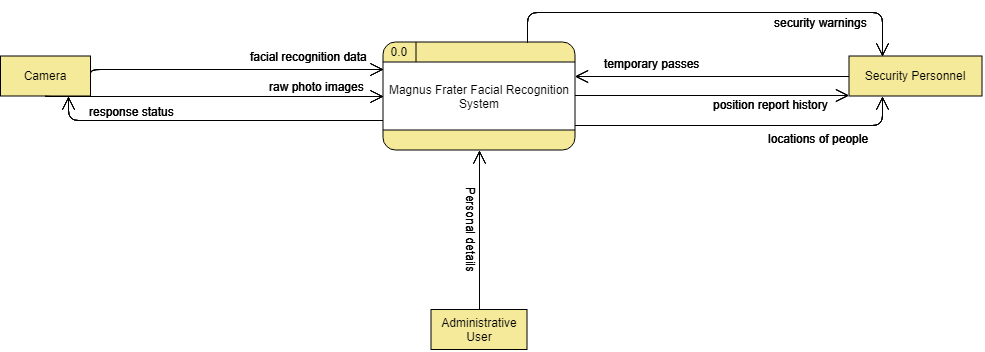
\includegraphics{images/ppm-images/context-diagram.png}
\caption{Context Diagram}
\end{figure}

\newpage

\begin{landscape}

\pagestyle{empty}

\hypertarget{level0dfd}{%
\section{Level 0 DFD}\label{level0dfd}}

\begin{figure}
    \makebox[\linewidth]{
        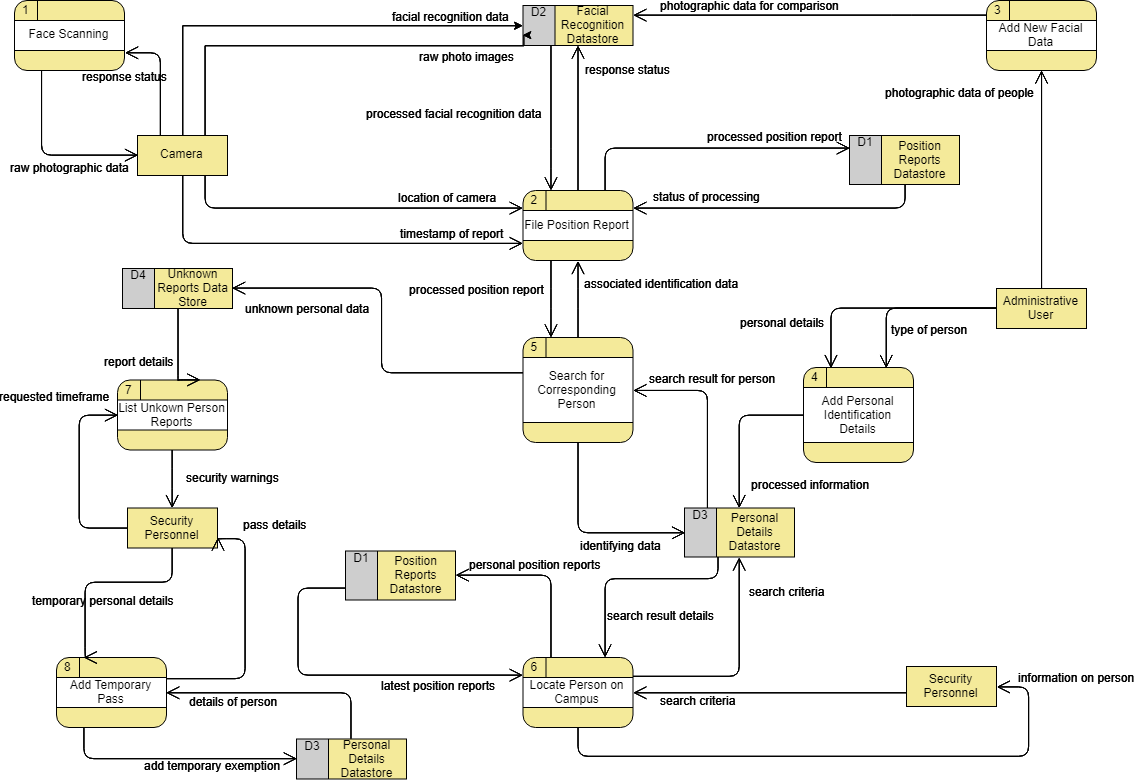
\includegraphics[width=0.90\linewidth]{images/ppm-images/level-0-dfd.png}
    }
    \caption{Level 0 DFD} \label{fig:level0dfd}
\end{figure}

\end{landscape}

\newpage

\begin{landscape}

\pagestyle{empty}

\hypertarget{cmap}{%
\section{Concept Map}\label{cmap}}

\begin{figure}
    \makebox[\linewidth]{
        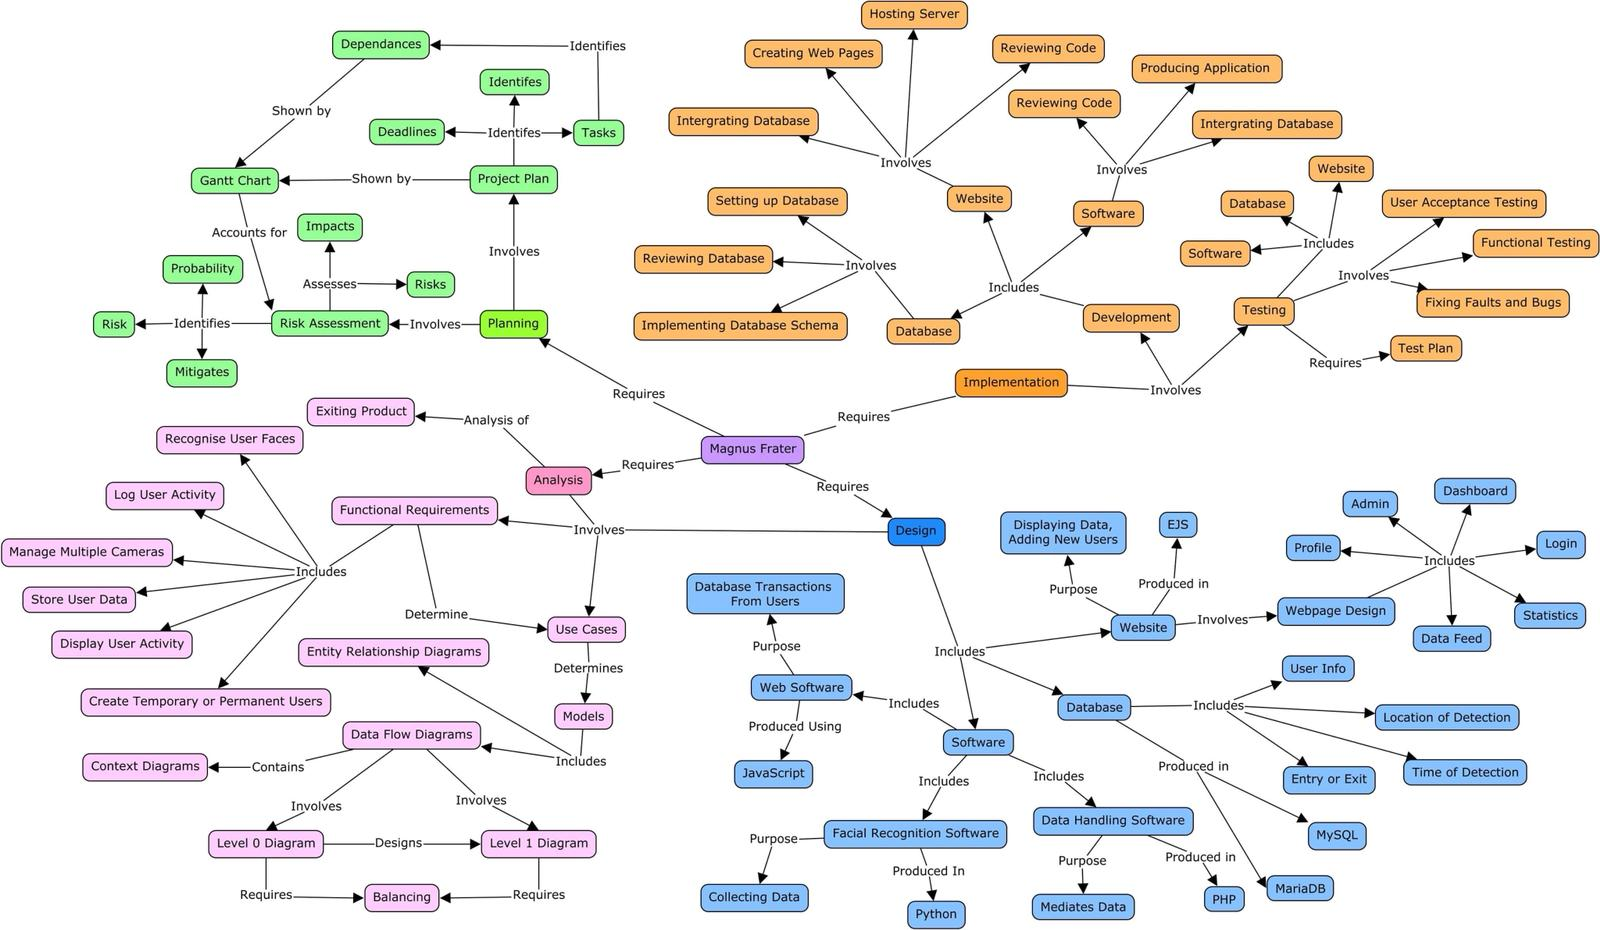
\includegraphics[width=1.05\linewidth]{images/ppm-images/cmap.jpeg}
    }
    \caption{Concept Map} \label{fig:cmap}
\end{figure}

\end{landscape}

\newpage

\hypertarget{bcs-code-of-conduct}{%
\subsection{BCS Code of Conduct}\label{bcs-code-of-conduct}}

In order to make our project as efficient as possible, the group decided
that it will essential to use the British Computer Society's (BCS) code
of conduct, so it can guide us with professional standards and be aware
of our responsibilities to each other and the public.

All of our decisions were made with the BCS code of conduct in mind. In
order to keep our work professional, with competence and integrity, we
made sure to thoroughly research and be up to date with the latest
technology and techniques for our respective parts in this project. As
it states in the BCS code of conduct \enquote{develop your professional
knowledge, skills and competence on a continuing basis, maintaining
awareness of technological developments, procedures, and standards that
are relevant to your field.} (``BCS Code of Conduct'' 2015).

Because of the nature of this project, working in a group, we ensured
that everyone in the group had the same rights and authority toward the
project. Everyone's thoughts and opinions were taken into account , no
matter the content, everyone had a voice and no one could contradict
that, not only it is immoral it is enforced by the (BCS) code of conduct
\enquote{respect and value alternative viewpoints and, seek, accept and
offer honest criticisms of work.} (``BCS Code of Conduct'' 2015).

With that said this brings us to another matter, any form of
discrimination was prohibited, not only it's immoral, it is also
illegal. The Equality Act 2010 and the BCS code of conduct state that
any kind of discrimination is not allowed \enquote{conduct your
professional activities without discrimination on the grounds of sex,
sexual orientation, marital status, nationality, colour, race, ethnic
origin, religion, age or disability, or of any other condition or
requirement} (``BCS Code of Conduct'' 2015).

It is important to say that we worked on this project for the public
interest. We wanted to provide security and efficiency. With this
product we want to saver time for the public and make there lives
easier. Of course, the privacy of the public is our priority, we
implemented restricted access to our product, so only personal that have
a username and password can access the private data. With the BCS code
of conduct stating, \enquote{You shall have due regard for public
health, privacy, security and wellbeing of others and the environment.}
(``BCS Code of Conduct'' 2015).

\newpage

\hypertarget{references}{%
\section*{References}\label{references}}
\addcontentsline{toc}{section}{References}

\hypertarget{refs}{}
\leavevmode\hypertarget{ref-bcs}{}%
``BCS Code of Conduct.'' 2015. \emph{BCS}.
\url{https://www.bcs.org/membership/become-a-member/bcs-code-of-conduct/}.

\leavevmode\hypertarget{ref-doran1981there}{}%
Doran, George T. 1981. ``There'sa Smart Way to Write Management's Goals
and Objectives.'' \emph{Management Review} 70 (11): 35--36.

\leavevmode\hypertarget{ref-agencies_2018}{}%
Staff, The Guardian, and Agencies. 2018. ``YouTube Hq Shooting: Police
Identify Woman Who Opened Fire.'' \emph{The Guardian}. Guardian News;
Media.
\url{https://www.theguardian.com/technology/2018/apr/04/youtube-shooting-police-identify-woman-opened-fire-hq}.

\end{document}
